\documentclass[conference]{IEEEtran}
\usepackage[utf8]{inputenc}
\usepackage{amsmath,amssymb}
\usepackage{graphicx}
\usepackage{booktabs}
\usepackage{cite}
\usepackage{url}
\usepackage[hidelinks]{hyperref}

\graphicspath{{../reports/paper/}}

\begin{document}

\title{Can Machine Learning Beat a Random Walk in Bitcoin? A Leakage-Free Benchmark of 32 Models}

\author{\IEEEauthorblockN{Rodayna Emad Mohamed}
\IEEEauthorblockA{College of Computer Science and Artificial Intelligence\\
Pharos University in Alexandria, Alexandria, Egypt\\
rodynaemad@gmail.com}}

\maketitle

\begin{abstract}
Machine learning studies of Bitcoin frequently report high forecasting accuracy, yet many evaluate on price levels, use leaky train/test splits, test on a single window, or ignore the number of models tried. We benchmark 32 forecasting models from six families against the random-walk (zero-return) forecast for 1-day and 7-day log returns: statistical models, linear and regularized regression, kernel methods, tree ensembles, gradient boosting and ten deep-learning architectures. All models share the same 66 leakage-guarded features and the same purged, embargoed, expanding-window walk-forward protocol, evaluated on 13 folds covering seven years (September 2019 to September 2026) of daily data. After Holm correction for multiple comparisons, \emph{no} model is significantly more accurate than the zero forecast at either horizon (Diebold--Mariano test), whereas 23 of 32 (1-day) and 25 of 32 (7-day) are significantly \emph{worse}, with error growing with model flexibility. Directional accuracy peaks at 51.1\% and is indistinguishable from a coin flip. In cost-aware backtests, 1 of 60 trading strategies edges past buy-and-hold on Sharpe ratio, and its deflated Sharpe ratio of 0.05 marks it as a likely artefact of multiple trials. Removing non-stationary price-level features improves most models but still leaves none better than the random walk. We release the frozen dataset, code and all out-of-sample predictions so the results can be reproduced exactly.
\end{abstract}

\begin{IEEEkeywords}
Bitcoin, cryptocurrency, time-series forecasting, machine learning, deep learning, market efficiency, walk-forward validation, data leakage, reproducibility, Diebold--Mariano test
\end{IEEEkeywords}

\section{Introduction}
\label{sec:intro}
Bitcoin is a popular target for machine learning: its data are free, it trades around the clock, and its large price swings appear to invite prediction. A substantial literature reports LSTM, gradient boosting and hybrid models forecasting its price with high accuracy. Such results are hard to compare and often hard to trust. Evaluating on price levels rewards a model for repeating yesterday's price; random train/test splits let a model learn from the future \cite{bergmeir2012, kapoor2023}; a single test window can coincide with one favourable market regime; and when dozens of architectures or hyperparameter settings are tried, the best one will look good by chance alone \cite{harvey2016, bailey2014}.

This paper asks a simple question under conditions designed to make the answer credible: \emph{when evaluated without leakage, over many market regimes, against the right benchmark and with corrections for multiple testing, does any standard forecasting model beat a random walk in Bitcoin?} Our contributions are:
\begin{enumerate}
  \item \textbf{A broad, uniform benchmark.} We evaluate 32 models from six families, from ARIMA and ridge regression to XGBoost, LSTMs and Transformers, on identical features and identical walk-forward folds, at 1-day and 7-day horizons.
  \item \textbf{A leakage-free protocol.} Features are lagged by construction and checked by unit tests; validation is expanding-window walk-forward with purging and embargo \cite{lopezdeprado2018}; only folds with at least two years of training history are scored.
  \item \textbf{Inference that accounts for the search.} We test every model against the random walk with the Diebold--Mariano test, adjust all $p$-values for multiple comparisons, and deflate the best backtest's Sharpe ratio for the number of strategies tried.
  \item \textbf{A clear negative result, released in full.} No model significantly beats the random walk; most are significantly worse, and error grows with model flexibility. The dataset snapshot, code and every out-of-sample prediction are public.
\end{enumerate}

Negative results are informative. They set a realistic baseline for future work, show how much apparent accuracy disappears under rigorous evaluation, and help practitioners avoid costly over-confidence.

\begin{figure*}[t]
  \centering
  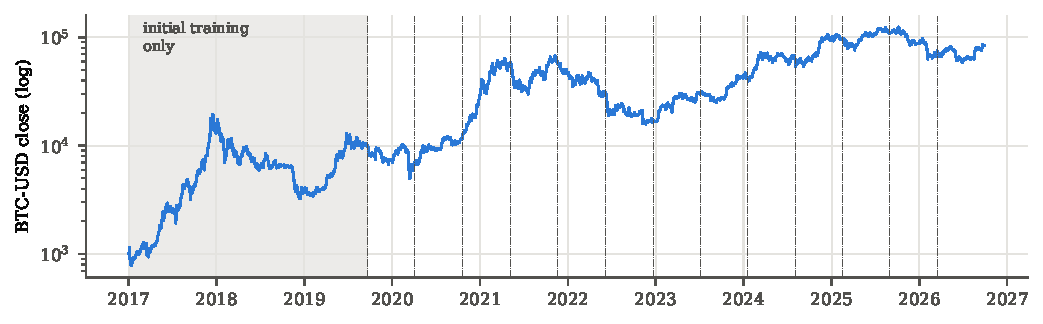
\includegraphics[width=\textwidth]{fig_price_folds.pdf}
  \caption{BTC-USD daily close (log scale). The shaded region is used only for initial training (including a 200-day indicator warm-up); dotted lines mark the starts of the 13 scored walk-forward test folds.}
  \label{fig:price}
\end{figure*}

\section{Related Work}
\label{sec:related}

\textbf{Market efficiency and Bitcoin.} The efficient market hypothesis \cite{fama1970} implies that publicly available price information cannot be used to forecast returns reliably. For Bitcoin, early evidence pointed to inefficiency \cite{urquhart2016}, but simple transformations of returns already restored weak-form efficiency in follow-up tests \cite{nadarajah2017}, and Urquhart himself reported that the market was becoming more efficient over time. This tension makes Bitcoin a natural test bed: if machine learning has an exploitable edge anywhere, a young, retail-heavy, 24/7 market is a plausible candidate.

\textbf{Machine learning for Bitcoin forecasting.} A large literature applies LSTMs, gradient boosting and other learners to Bitcoin prices, often reporting high accuracy (e.g., \cite{mcnally2018}). Jaquart et al.~\cite{jaquart2021} compare several model classes on short horizons and find predictability that is statistically detectable but small and largely eroded by transaction costs. Many studies, however, evaluate on price levels, where predicting yesterday's price already yields low error; use random train/test splits that leak future information; report a single test window; or compare a proposed model only against weak or untuned alternatives. Kapoor and Narayanan \cite{kapoor2023} document how such data leakage has inflated published results across machine-learning-based science.

\textbf{Evaluation methodology.} We draw on established forecasting and finance practice. Out-of-sample $R^2$ against a naive benchmark \cite{campbell2008, welch2008} measures whether a model beats the random walk. The Diebold--Mariano test \cite{diebold1995} assesses whether accuracy differences are statistically significant. Purged and embargoed walk-forward validation \cite{lopezdeprado2018} prevents leakage through overlapping labels, and cross-validation for time series requires respecting temporal order \cite{bergmeir2012}. When many models or strategies are compared, multiple-testing corrections \cite{holm1979, harvey2016} and the deflated Sharpe ratio \cite{bailey2014} guard against declaring the luckiest backtest a discovery.

Our contribution is to combine these safeguards in a single, open, reproducible benchmark spanning 32 models from six families plus the random walk, evaluated on the same leakage-free folds over seven years that include several distinct market regimes.

\section{Data and Experimental Protocol}
\label{sec:method}

\subsection{Data}
We use daily BTC-USD open, high, low, close and volume (OHLCV) candles from Yahoo Finance covering 1~January~2017 to 30~September~2026 (3{,}560 days). The series is frozen as a CSV snapshot that ships with the code, so every number in this paper can be regenerated exactly. Bitcoin trades every day, so no calendar gaps are filled. Over the sample the price ranges from roughly \$778 to \$124{,}753, spanning the 2017 bubble, the 2018 and 2022 bear markets, the March~2020 crash, the 2021 bull market and the post-2024 spot-ETF era (Fig.~\ref{fig:price}).

\subsection{Prediction targets}
For horizon $h \in \{1, 7\}$ days the target is the forward log return
\begin{equation}
  y_t^{(h)} = \ln P_{t+h} - \ln P_t ,
\end{equation}
where $P_t$ is the daily close. We predict returns rather than price levels because a model that simply repeats yesterday's price attains a deceptively low price-level error while carrying no information; on returns, that same model is the zero forecast $\hat y_t = 0$, which becomes our principal benchmark.

\subsection{Features}
All models receive the same 66 features computed from OHLCV alone: 14 lagged log returns; rolling mean, standard deviation, skewness and kurtosis of returns over 7, 14, 30 and 90 days; realized, Parkinson and Garman--Klass volatility; rate of change and a 30-day price $z$-score; standard technical indicators (RSI, MACD, Bollinger bandwidth and \%B, ATR, ADX, CCI, Williams \%R, stochastic oscillator, on-balance volume, VWAP distance, 9/21/50/200-day EMAs and SMAs and their crossovers); and regime descriptors (drawdown from all-time high, a 200-day moving-average bull/bear flag, days since the last halving, a rolling Hurst exponent and an expanding-window volatility tercile).

\textbf{Leakage guard.} Every feature is first computed from data available up to and including day $t$, and the \emph{entire} feature block is then shifted forward by one day, so the row used to forecast $y_t^{(h)}$ contains only information known at the close of day $t-1$. Automated unit tests in the repository verify both the shift and that perturbing future prices leaves every past feature row unchanged.

\subsection{Models}
We evaluate the zero forecast plus 32 regression models, grouped below, all through one shared \texttt{fit}/\texttt{predict} interface:
\begin{itemize}
  \item \textbf{Baselines (3):} zero return (random walk), training-set mean return, and a constant small positive return (``always long'').
  \item \textbf{Statistical (3):} auto-ARIMA \cite{hyndman2008}, Holt--Winters exponential smoothing and Prophet \cite{taylor2018}, each fitted on the return series alone.
  \item \textbf{Linear (7):} lag-1 OLS, OLS on all features, ridge, lasso, elastic net, Bayesian ridge and Huber regression.
  \item \textbf{Kernel and instance-based (2):} support vector regression and $k$-nearest neighbours.
  \item \textbf{Tree ensembles and boosting (8):} decision tree, random forest, extra trees, AdaBoost, scikit-learn gradient boosting \cite{pedregosa2011}, XGBoost \cite{chen2016}, LightGBM \cite{ke2017} and CatBoost \cite{prokhorenkova2018}.
  \item \textbf{Deep learning (10):} MLP, vanilla RNN, LSTM \cite{hochreiter1997}, GRU, bidirectional LSTM, 1-D CNN, CNN--LSTM, LSTM with attention, a Transformer encoder \cite{vaswani2017} and a temporal convolutional network \cite{bai2018}. Each reads a 30-day window of the feature vector.
\end{itemize}
Classical and boosting models use library defaults; features are standardized inside each training fold. Deep models are trained with Adam (learning rate $10^{-3}$), mean-squared-error loss, batch size 64, gradient clipping at 1.0, up to 50 epochs with early stopping (patience 5) on the chronologically last 15\% of each training fold. We deliberately do not tune hyperparameters on the test periods: with 32 models, per-model tuning against the same history is itself a source of selection bias \cite{bailey2014}.

\subsection{Purged walk-forward validation}
Random $k$-fold cross-validation is invalid for this problem because it trains on the future \cite{bergmeir2012}. We instead use expanding-window walk-forward validation. The 3{,}359 usable rows at $h=1$ (3{,}353 at $h=7$, after indicator warm-up) are split into 17 contiguous blocks; fold $i$ tests on block $i$ and trains on everything before it. Two safeguards from \cite{lopezdeprado2018} remove leakage through overlapping targets: the $h$ rows immediately before each test block are \emph{purged} from training, because their targets extend into the test period, and the $h$ rows after each earlier test block are \emph{embargoed}. We only score folds with at least two years (730 rows) of training history. This leaves 13 test folds of about 198 days each, from September~2019 to September~2026, for a total of 2{,}567 one-day and 2{,}561 seven-day out-of-sample forecasts per model. Every model sees the same folds.

Sequence models need 30 days of input history even for the first day of a test block. Rather than padding, we pass the real preceding 29 feature rows as context. Their features are known before the test block begins, so this adds no information about the targets.

Statistical models (ARIMA, Holt--Winters, Prophet) are refitted once per fold and forecast the whole $\sim$198-day block from the end of training, whereas feature-based models update their inputs daily. This favours feature-based models, so it cannot explain any failure of theirs to beat the baselines.

\subsection{Evaluation}
\textbf{Forecast accuracy.} We report RMSE, MAE and the out-of-sample $R^2$ of Campbell and Thompson \cite{campbell2008} relative to the zero forecast,
\begin{equation}
  R^2_{OS} = 1 - \frac{\sum_t (y_t - \hat y_t)^2}{\sum_t y_t^2},
\end{equation}
which is positive only if a model beats the random walk in mean squared error.

\textbf{Equal predictive accuracy.} For each model we test equal mean squared error against the zero forecast with the Diebold--Mariano (DM) test \cite{diebold1995}, using a Newey--West variance with $h-1$ lags to account for the serial correlation that overlapping 7-day targets induce.

\textbf{Directional accuracy.} We report the share of days on which the predicted sign matches the realized sign. For $h=1$ (non-overlapping targets) we test it against a coin flip with a one-sided binomial test.

\textbf{Multiple testing.} Because 32 models are compared against the same benchmark, we adjust all $p$-values with the Holm--Bonferroni procedure \cite{holm1979} and treat only adjusted $p<0.05$ as evidence \cite{harvey2016}.

\textbf{Economic value.} For $h=1$ we convert each model's forecast into a daily position, either long/short ($\mathrm{sign}(\hat y_t)$) or long/flat ($\max(0, \mathrm{sign}(\hat y_t))$), and backtest it with a 0.10\% fee plus 0.05\% slippage charged on every unit of position change. We compare annualized Sharpe ratios (365 periods per year), compound annual growth and maximum drawdown with buy-and-hold, and we correct the best strategy's Sharpe ratio for the number of strategies tried using the deflated Sharpe ratio (DSR) of Bailey and L\'opez de Prado \cite{bailey2014}.


\begin{table*}[t]
\centering
\caption{Out-of-sample forecast accuracy, 13 walk-forward folds (Sep.~2019--Sep.~2026). $R^2_{OS}$ is relative to the zero-return forecast (\%). DM is the Diebold--Mariano statistic against the zero forecast (positive = less accurate); $p_{\mathrm{Holm}}$ is Holm-adjusted over 32 models. DA is directional accuracy (\%). Bold $R^2_{OS}$ marks the only positive values; none is significant.}
\label{tab:main}
\small
\begin{tabular}{llrrrrrrr}
\toprule
 & & \multicolumn{4}{c}{1-day horizon} & \multicolumn{3}{c}{7-day horizon} \\
\cmidrule(lr){3-6}\cmidrule(lr){7-9}
Family & Model & $R^2_{OS}$ & DA & DM & $p_{\mathrm{Holm}}$ & $R^2_{OS}$ & DM & $p_{\mathrm{Holm}}$ \\
\midrule
Baseline & Always long & \textbf{+0.02} & 50.4 & -1.24 & 1.000 & \textbf{+0.02} & -1.66 & 0.584 \\
 & Zero return (random walk) & 0 & -- & -- & -- & 0 & -- & -- \\
 & Mean return & -0.06 & 50.4 & 0.35 & 1.000 & -0.58 & 0.51 & 1.000 \\
\addlinespace[2pt]
Statistical & Auto-ARIMA & -0.02 & 50.1 & 0.16 & 1.000 & -1.06 & 1.74 & 0.570 \\
 & Holt--Winters & -0.55 & 49.9 & 2.24 & 0.201 & -41.40 & 5.04 & $<$0.001 \\
 & Prophet & -3.97 & 50.8 & 4.64 & $<$0.001 & -31.00 & 5.68 & $<$0.001 \\
\addlinespace[2pt]
Linear & Lag-1 OLS & \textbf{+0.10} & 49.5 & -0.39 & 1.000 & -0.60 & 0.54 & 1.000 \\
 & Elastic net & -0.06 & 50.4 & 0.35 & 1.000 & -0.58 & 0.51 & 1.000 \\
 & Lasso & -0.06 & 50.4 & 0.35 & 1.000 & -0.58 & 0.51 & 1.000 \\
 & Bayesian ridge & -11.40 & 49.7 & 6.16 & $<$0.001 & -256 & 4.52 & $<$0.001 \\
 & Huber & -60.83 & 49.7 & 11.50 & $<$0.001 & -617 & 5.13 & $<$0.001 \\
 & Ridge & -146 & 49.8 & 11.60 & $<$0.001 & -651 & 5.93 & $<$0.001 \\
 & OLS (all features) & -202 & 49.5 & 13.47 & $<$0.001 & -1036 & 6.26 & $<$0.001 \\
\addlinespace[2pt]
Kernel & $k$-NN & -33.60 & 48.7 & 12.10 & $<$0.001 & -103 & 9.36 & $<$0.001 \\
 & SVR & -34.47 & 50.6 & 12.95 & $<$0.001 & -80.17 & 9.06 & $<$0.001 \\
\addlinespace[2pt]
Tree ensemble & AdaBoost & -10.73 & 48.3 & 6.95 & $<$0.001 & -42.65 & 5.93 & $<$0.001 \\
 & Random forest & -37.34 & 51.1 & 11.86 & $<$0.001 & -104 & 7.73 & $<$0.001 \\
 & Extra trees & -39.08 & 50.3 & 11.54 & $<$0.001 & -57.35 & 6.80 & $<$0.001 \\
 & Decision tree & -335 & 49.8 & 25.84 & $<$0.001 & -368 & 9.02 & $<$0.001 \\
\addlinespace[2pt]
Gradient boosting & CatBoost & -0.42 & 48.4 & 1.50 & 0.928 & -0.55 & 0.79 & 1.000 \\
 & LightGBM & -0.88 & 49.8 & 2.60 & 0.084 & -6.25 & 4.69 & $<$0.001 \\
 & XGBoost & -9.93 & 48.1 & 7.62 & $<$0.001 & -29.10 & 6.50 & $<$0.001 \\
 & Gradient boosting & -132 & 49.6 & 12.75 & $<$0.001 & -145 & 7.92 & $<$0.001 \\
\addlinespace[2pt]
Deep learning & Transformer & -39.24 & 48.5 & 15.43 & $<$0.001 & -26.23 & 4.55 & $<$0.001 \\
 & CNN--LSTM & -52.57 & 50.1 & 10.73 & $<$0.001 & -141 & 6.87 & $<$0.001 \\
 & TCN & -110 & 49.4 & 11.27 & $<$0.001 & -198 & 4.78 & $<$0.001 \\
 & LSTM + attention & -254 & 51.1 & 19.99 & $<$0.001 & -85.18 & 7.13 & $<$0.001 \\
 & BiLSTM & -451 & 49.0 & 14.93 & $<$0.001 & -197 & 6.68 & $<$0.001 \\
 & LSTM & -512 & 50.2 & 20.38 & $<$0.001 & -222 & 7.89 & $<$0.001 \\
 & RNN & -596 & 47.0 & 19.48 & $<$0.001 & -290 & 7.48 & $<$0.001 \\
 & GRU & -1023 & 50.7 & 18.62 & $<$0.001 & -345 & 6.91 & $<$0.001 \\
 & 1-D CNN & -4374 & 50.1 & 13.13 & $<$0.001 & -264 & 7.90 & $<$0.001 \\
 & MLP & -9319 & 49.4 & 22.56 & $<$0.001 & -2904 & 7.75 & $<$0.001 \\
\bottomrule
\end{tabular}
\end{table*}


\begin{figure*}[t]
  \centering
  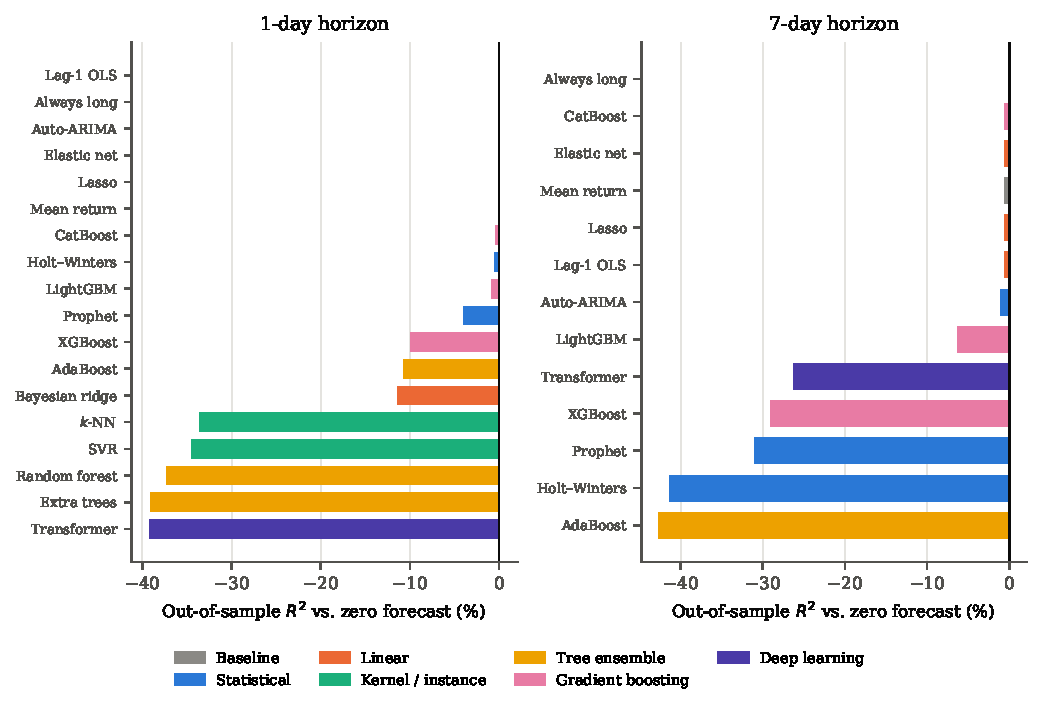
\includegraphics[width=\textwidth]{fig_r2_os.pdf}
  \caption{Out-of-sample $R^2$ relative to the zero-return forecast. Bars left of zero are less accurate than predicting no change. For readability, models with $R^2_{OS} < -50\%$ are omitted: 14 models at 1 day and 19 at 7 days, including every deep-learning model except the Transformer (see Table~\ref{tab:main}).}
  \label{fig:r2}
\end{figure*}

\section{Results}
\label{sec:results}

Each model produces 2{,}567 one-day and 2{,}561 seven-day out-of-sample forecasts over 13 folds from 20~September~2019 to 29~September~2026. No model failed on any fold.

\subsection{Forecast accuracy: no model beats the random walk}
Table~\ref{tab:main} and Fig.~\ref{fig:r2} summarize forecast accuracy. At the one-day horizon only two of the 32 models have a positive out-of-sample $R^2$: lag-1 OLS ($R^2_{OS} = 0.10\%$) and the constant ``always long'' forecast ($0.02\%$). Neither improvement is statistically meaningful (DM $p = 0.70$ and $0.22$ before any correction). At the seven-day horizon only the ``always long'' forecast is positive ($0.02\%$, DM $p = 0.10$, Holm-adjusted $p = 0.58$). \textbf{After the Holm correction, zero models are significantly more accurate than the zero forecast at either horizon.}

The opposite is not true. Twenty-three of 32 models at $h=1$ and 25 of 32 at $h=7$ are significantly \emph{less} accurate than the zero forecast after correction. The models that escape this are exactly those whose forecasts stay close to zero: the trivial baselines, auto-ARIMA, lag-1 OLS, lasso, elastic net and CatBoost at both horizons, plus LightGBM and Holt--Winters at $h=1$ only. With library-default regularization, lasso and elastic net shrink every coefficient to zero and reproduce the mean-return baseline exactly; the regularizer itself finds no usable linear signal. Accuracy falls as model flexibility grows. The median $R^2_{OS}$ by family at $h=1$ is $-0.6\%$ for statistical models, $-5.4\%$ for gradient boosting, $-11\%$ for linear models, $-34\%$ for kernel methods, $-38\%$ for tree ensembles and $-481\%$ for deep learning. Fourteen models at $h=1$ and nineteen at $h=7$ have $R^2_{OS} < -50\%$, meaning their errors are substantially larger than those of predicting no change at all.

\subsection{Directional accuracy is indistinguishable from a coin flip}
At $h=1$, directional accuracy ranges from 47.0\% (RNN) to 51.1\% (random forest and LSTM with attention); 14 of 32 models exceed 50\% (Fig.~\ref{fig:da}). The most favourable one-sided binomial test, for random forest, gives $p = 0.13$ \emph{before} correction; after correction no model differs from 50\%. Stability across time is also absent. The five highest-accuracy models beat 50\% in only 7 to 9 of the 13 folds, roughly what chance alone produces.

At $h=7$ the highest directional accuracy, 54.4\% for Holt--Winters, is a base-rate artefact rather than skill. Bitcoin rose in 52.8\% of the overlapping seven-day windows, Holt--Winters predicts a rise 61.5\% of the time, and its $R^2_{OS}$ is $-41\%$. A constant ``always up'' forecast attains 52.8\% at no cost.

\subsection{Economic value: one of 60 strategies edges past buy-and-hold}
Table~\ref{tab:backtest} and Fig.~\ref{fig:equity} report the cost-aware backtests at $h=1$. Buying and holding Bitcoin over the test period earned a compound annual growth rate (CAGR) of 34.9\% with a Sharpe ratio of 0.80 and a maximum drawdown of $-76.6\%$. Of the 60 model-driven strategies (30 non-trivial models $\times$ long/short and long/flat), none of the long/short strategies beats buy-and-hold on Sharpe ratio, and their median Sharpe is $-0.45$. Long/flat strategies fare better (median 0.25), because they inherit Bitcoin's upward drift whenever they are invested, but only one, GRU long/flat, exceeds buy-and-hold: Sharpe 0.82 versus 0.80, with a lower CAGR (25.6\%) and a shallower drawdown ($-54.4\%$).

That single success is what chance predicts when 60 strategies are tried. Correcting the GRU's Sharpe ratio for the number of trials, the variance of Sharpe ratios across trials and the non-normality of its returns gives a deflated Sharpe ratio of 0.05, far below the 0.95 needed to call it a discovery \cite{bailey2014}. Its curve in Fig.~\ref{fig:equity} also shows long flat stretches out of the market rather than consistent timing.


\begin{figure}[t]
  \centering
  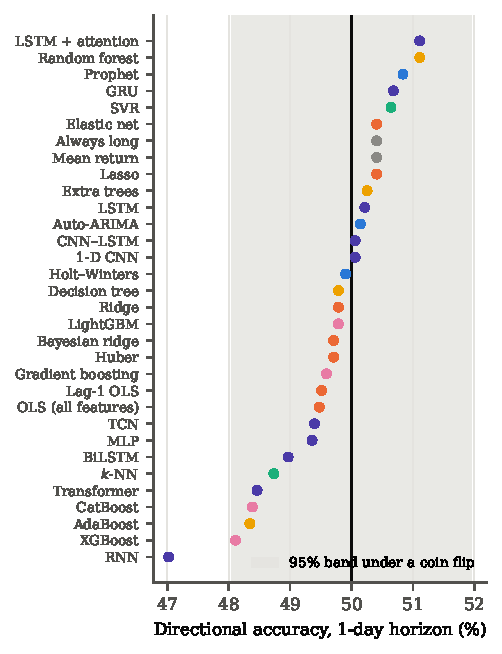
\includegraphics[width=\columnwidth]{fig_dir_acc.pdf}
  \caption{One-day directional accuracy of each model. The shaded band is the 95\% range expected from a fair coin over the same number of forecasts; every model except the RNN (47.0\%, below the band) lies inside it.}
  \label{fig:da}
\end{figure}

\begin{table}[t]
\centering
\caption{Cost-aware backtests of 1-day forecasts (0.10\% fee + 0.05\% slippage per unit of position change). Top six trading strategies by Sharpe ratio and medians over all 60 model-driven strategies. L/F = long/flat, L/S = long/short, DD = maximum drawdown, Turn. = mean daily turnover.}
\label{tab:backtest}
\footnotesize
\setlength{\tabcolsep}{3.5pt}
\begin{tabular}{lrrrr}
\toprule
Strategy & Sharpe & CAGR\% & DD\% & Turn. \\
\midrule
Buy \& hold & 0.80 & 34.9 & -76.6 & 0.00 \\
\midrule
GRU (L/F) & 0.82 & 25.6 & -54.4 & 0.12 \\
SVR (L/F) & 0.79 & 29.3 & -58.4 & 0.09 \\
Random forest (L/F) & 0.68 & 18.2 & -56.0 & 0.17 \\
MLP (L/F) & 0.65 & 20.1 & -57.0 & 0.05 \\
LSTM + attention (L/F) & 0.58 & 16.9 & -59.5 & 0.02 \\
LightGBM (L/F) & 0.56 & 16.5 & -70.8 & 0.08 \\
\midrule
Median L/S (n=30) & -0.45 & -36.0 & -97.6 & 0.23 \\
Median L/F (n=30) & 0.25 & 2.0 & -70.8 & 0.12 \\
\bottomrule
\end{tabular}
\end{table}


\begin{figure*}[t]
  \centering
  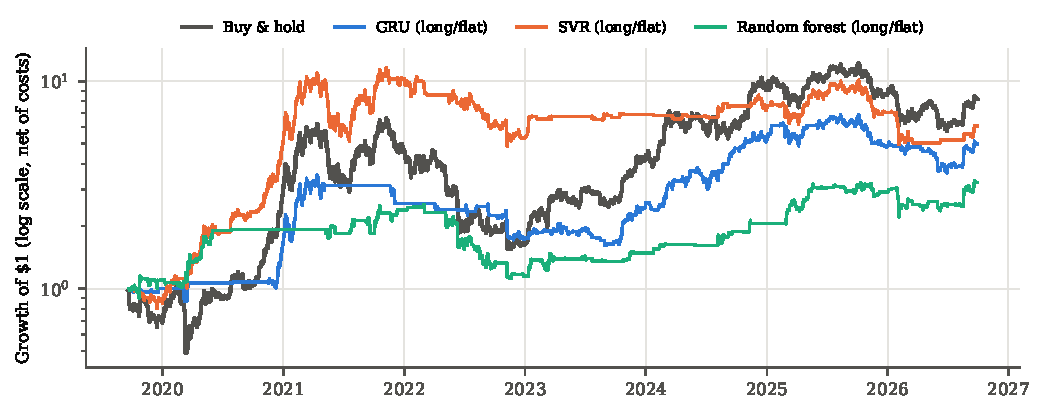
\includegraphics[width=\textwidth]{fig_equity.pdf}
  \caption{Growth of \$1, net of costs, for buy-and-hold and the three highest-Sharpe actively trading strategies (log scale). Flat segments are periods out of the market.}
  \label{fig:equity}
\end{figure*}

\section{Robustness: Removing Non-Stationary Features}
\label{sec:robust}

Thirteen of the 66 features are measured in price units: four EMAs, four SMAs, MACD and its signal and histogram, ATR and on-balance volume. Because Bitcoin rose more than tenfold from the start of the test period to its peak, their test-fold values often lie outside anything seen in training. To check whether these features alone drive the poor results, we re-ran 16 representative models at $h=1$ using only the 53 remaining, scale-free features. The rows, folds and protocol are exactly the same as in the main run.

Table~\ref{tab:robust} shows that the price-level features explain a large part of the damage but not the absence of skill. Removing them improves $R^2_{OS}$ for 14 of the 16 models and raises the median from $-45.8\%$ to $-16.7\%$, with the largest gains for linear models, tree ensembles and recurrent networks. Yet \emph{no} model reaches a positive $R^2_{OS}$, none is significantly better than the zero forecast, and 13 of the 16 remain significantly worse after Holm correction (versus 15 of 16 with all features). The best directional accuracy, 51.4\% for XGBoost, is again not significant (one-sided binomial $p = 0.08$ before correction). The main conclusion is therefore not an artefact of feature scaling.

\begin{table}[t]
\centering
\caption{Robustness: 1-day results with all 66 features vs.\ 53 stationary features (13 price-level features removed). $R^2_{OS}$ in \%; $p_{\mathrm{Holm}}$ from the DM test against the zero forecast, adjusted over the 16 models shown; DA in \%.}
\label{tab:robust}
\footnotesize
\setlength{\tabcolsep}{3.5pt}
\begin{tabular}{lrrrrr}
\toprule
 & \multicolumn{2}{c}{All features} & \multicolumn{3}{c}{Stationary only} \\
\cmidrule(lr){2-3}\cmidrule(lr){4-6}
Model & $R^2_{OS}$ & $p_{\mathrm{Holm}}$ & $R^2_{OS}$ & $p_{\mathrm{Holm}}$ & DA \\
\midrule
CatBoost & -0.42 & 0.133 & -0.31 & 0.233 & 49.2 \\
LightGBM & -0.88 & 0.019 & -0.70 & 0.233 & 49.6 \\
XGBoost & -9.93 & $<$0.001 & -12.22 & $<$0.001 & 51.4 \\
Bayesian ridge & -11.40 & $<$0.001 & -0.79 & 0.233 & 48.7 \\
$k$-NN & -33.60 & $<$0.001 & -33.87 & $<$0.001 & 50.7 \\
SVR & -34.47 & $<$0.001 & -34.33 & $<$0.001 & 49.5 \\
Random forest & -37.34 & $<$0.001 & -15.59 & $<$0.001 & 49.1 \\
Extra trees & -39.08 & $<$0.001 & -10.46 & $<$0.001 & 50.0 \\
CNN--LSTM & -52.57 & $<$0.001 & -17.23 & $<$0.001 & 48.7 \\
Huber & -60.83 & $<$0.001 & -15.14 & $<$0.001 & 49.4 \\
TCN & -110 & $<$0.001 & -16.21 & $<$0.001 & 49.1 \\
Ridge & -146 & $<$0.001 & -47.02 & $<$0.001 & 48.3 \\
OLS (all features) & -202 & $<$0.001 & -48.43 & $<$0.001 & 48.0 \\
LSTM & -512 & $<$0.001 & -195 & $<$0.001 & 49.8 \\
GRU & -1023 & $<$0.001 & -234 & $<$0.001 & 49.7 \\
MLP & -9319 & $<$0.001 & -1744 & $<$0.001 & 50.3 \\
\bottomrule
\end{tabular}
\end{table}


\section{Discussion}
\label{sec:discussion}

\textbf{Why does flexibility hurt?} Daily Bitcoin returns have a standard deviation of about 3\%, while any predictable component is, at best, a small fraction of that. With so little signal relative to noise, a model's error is dominated by its variance: every unit of flexibility spent fitting noise in the training folds is paid back out of sample. Models that predict values close to zero (the baselines, heavily shrunk linear models, auto-ARIMA and conservatively regularized boosting such as CatBoost) cannot lose much, while unconstrained learners such as deep networks, fully grown trees and unregularized OLS lose a great deal. This echoes Welch and Goyal's finding for equity premium prediction \cite{welch2008}, where predictors that look useful in sample routinely fail out of sample. It also means that a model that ``wins'' on an in-sample or single-window evaluation is more likely to be the one that overfitted most.

\textbf{Non-stationarity.} Bitcoin's price rose more than tenfold from the start of the evaluation period to its peak. Features measured in price units (moving averages, MACD, ATR, on-balance volume) therefore take values in the test folds that never appeared in training, which tree-based and neural models cannot extrapolate. Section~\ref{sec:robust} shows how much of the damage this explains. It does not, however, create a positive result: even with stationary features, no model beats the random walk.

\textbf{Directional accuracy is a weak and misleading metric.} Accuracy near 50\% is easily reported as ``better than chance'' without a test. Over 2{,}567 forecasts, the 95\% range for a fair coin is roughly 48--52\%, wide enough to contain every model here except the RNN, which falls below it. At longer horizons, overlapping targets inflate the effective significance and a positive drift rewards models biased toward predicting rises, as the 54.4\% Holt--Winters figure illustrates. We recommend always reporting directional accuracy next to the base rate and an $R^2_{OS}$ against the zero forecast.

\textbf{Implications.} For researchers, a credible claim of predictability should (i) evaluate returns, not price levels; (ii) use walk-forward validation with purging; (iii) span several market regimes; (iv) compare against the zero forecast and buy-and-hold; (v) test significance and correct it for every model and setting tried; and (vi) account for transaction costs. For practitioners, the results caution that off-the-shelf models trained on price and volume data are unlikely to beat simply holding the asset.

\textbf{Limitations.} Our conclusions are bounded by our design. We use only OHLCV-derived features. On-chain activity, order-book, derivatives, macro-financial and sentiment data may contain information that price and volume do not, and the codebase already includes fetchers for several of them. We study daily data, a single asset and library-default hyperparameters; nested tuning within each training fold could help some models, although it would also widen the search that our corrections must account for. Statistical models forecast each test block from the end of training rather than updating daily. Deep models were trained on CPU with early stopping and a 50-epoch cap. Finally, our evaluation period is one realized history; a different seven years could favour different models, which is precisely why we report significance rather than rankings.


\section{Conclusion}
\label{sec:conclusion}
Under a leakage-free, multi-regime, multiple-testing-aware evaluation, none of 32 standard forecasting models, including ten deep-learning architectures and three gradient-boosting libraries, predicts daily or weekly Bitcoin returns significantly better than a random walk. Most do significantly worse, the more flexible the model the larger the damage, and the single trading strategy that edges past buy-and-hold does not survive a correction for the number of strategies tried. We do not claim that Bitcoin is unpredictable with every possible model or data source. We do claim that price-and-volume features combined with off-the-shelf learners do not yield a reliable edge, and that a credible positive claim must clear the bar set here: beat the zero forecast out of sample, across regimes, with significance that survives correction for the search. Future work will add exogenous data (on-chain activity, macro-financial series and sentiment), intraday frequencies and nested hyperparameter tuning within the same protocol.

\section*{Reproducibility}
{\raggedright
All code, the frozen data snapshot (\path{data/snapshots/}), every out-of-sample prediction (\path{reports/paper/oof_h*.csv}) and the scripts that generate each table and figure are available at \url{https://github.com/itsRou/bitcoin-price-prediction}. Running \path{scripts/run_real_benchmark.py} followed by \path{scripts/analyze_real_benchmark.py} and \path{scripts/make_paper_tables.py} regenerates every result, table and figure.\par}

\bibliographystyle{IEEEtran}
\bibliography{refs}

\end{document}
